% Indicate the main file. Must go at the beginning of the file.
% !TEX root = ../main.tex

%----------------------------------------------------------------------------------------
% EINLEITUNG
%----------------------------------------------------------------------------------------


\chapter{Einleitung} % Main chapter title
In der modernen Softwareentwicklung sind Code-Reviews ein essenzieller Bestandteil zur Sicherstellung der Codequalität sowie zur Förderung der Teamzusammenarbeit. In der Praxis erfolgen diese Reviews meist über Plattformen wie GitHub oder GitLab, wobei sogenannte Pull-Requests (auch Merge-Requests genannt) den strukturellen Rahmen für den Reviewprozess bilden.

Ein zentrales Problem in softwarebasierten Teamprojekten ist die fehlende Transparenz über die Qualität der Zusammenarbeit und den Zustand des Entwicklungsprozesses. Zwar liefern Pull-Requests wertvolle Daten, doch deren systematische Auswertung bleibt oft ungenutzt. Diese Problematik bildet den Ausgangspunkt der vorliegenden Arbeit. Durch die Analyse von Code-Review-Daten lassen sich frühzeitig technische Probleme sowie Herausforderungen in der Teamkoordination erkennen.

An der Zürcher Hochschule für Angewandte Wissenschaften (ZHAW) führen Studierende im Rahmen von vier Projektmodulen Softwareprojekte in Teams durch. Lehrpersonen stehen dabei vor der Herausforderung, die Teamleistung objektiv zu beurteilen. Eine automatisierte Auswertung der Code-Review-Daten bietet ihnen ein wirkungsvolles Instrument, um potenzielle Probleme frühzeitig zu identifizieren und gezielt zu intervenieren.

Zur Unterstützung dieser Auswertung wurde an der ZHAW das Tool \textit{GitGauge} entwickelt. GitGauge ist ein Repository-Mining- und Analysewerkzeug mit einer Web-Benutzeroberfläche.

Ziel der Arbeit ist es, GitGauge funktional zu erweitern, neue Metriken zu entwickeln und gezielte Analysen zu ermöglichen, die auf die spezifischen Anforderungen der Projektmodule abgestimmt sind. Damit soll ein praxisnahes Werkzeug entstehen, das sowohl Lehrpersonen als auch Studierenden neue Erkenntnisse über Teamdynamik und Arbeitsweise liefert.

Im Mittelpunkt der Untersuchung stehen sechs eigens entwickelte Forschungsfragen. Diese beleuchten unter anderem, ob ein Zusammenhang zwischen der Bearbeitungsdauer (Latency) eines Pull-Requests und der Anzahl geänderter Codezeilen (Churn) besteht, wie sich die Review-Dauer im zeitlichen Verlauf eines Projekts verändert und welche Unterschiede zwischen Vollzeit- und Teilzeitstudierenden hinsichtlich ihrer Pull-Request-Nutzung bestehen.

Die Arbeit ist wie folgt aufgebaut: Kapitel 2 erläutert die theoretischen Grundlagen, darunter Git-spezifische Konzepte, eine Einführung in die Projektmodule sowie das Tool GitGauge. Kapitel 3 beschreibt die methodische Vorgehensweise zur Beantwortung der Forschungsfragen. In Kapitel 4 werden die Ergebnisse präsentiert und diskutiert. Kapitel 5 fasst die Resultate zusammen und gibt einen Ausblick auf zukünftige Weiterentwicklungen.



\label{Chapter1} % Change X to a consecutive number; for referencing this chapter elsewhere, use \ref{ChapterX}

%----------------------------------------------------------------------------------------
% SECTION 1
%----------------------------------------------------------------------------------------

\section{Ausgangslage}
\label{sec:Ausgangslage} 
Code-Reviews sind ein wichtiger Bestandteil der modernen Softwareentwicklung. Reviews fördern nicht nur die Qualität des Codes, sondern auch die Zusammenarbeit im Team \parencite{dos_santos_investigating_2018}. In der Praxis werden Code-Reviews häufig über Plattformen wie GitHub oder GitLab durchgeführt \parencite{noauthor_team_nodate}. Dabei werden auf der Plattform sogenannte Pull-Requests / Merge-Requests erstellt, welche dann als Grundlage für die Reviews dienen. Die Bezeichnung kann sich von Plattform zu Plattform ändern, beschreibt aber jeweils dasselbe Konzept \parencite{kansab_analyzing_2025}.


Die Analyse der Code-Review-Daten kann wertvolle Informationen über die Zusammenarbeit und den Fortschritt innerhalb eines Softwareprojekts liefern. So kann beispielsweise festgestellt werden, wie oft bestimmte Contributor miteinander interagieren oder wie lange es durchschnittlich dauert, bis ein Review abgeschlossen ist. Eine automatisierte Auswertung bietet die Möglichkeit, Probleme oder Verbesserungsmöglichkeiten zu erkennen. Diese können sowohl auf technischer als auch auf sozialer Ebene sein. 

An der Zürcher Hochschule für Angewandte Wissenschaften (ZHAW) lernen die Studierenden in Projektmodulen, wie man Projekte erfolgreich durchführt. Für die Zusammenarbeit der Teams wird GitHub eingesetzt. Eine automatisierte Auswertung der Code-Reviews kann den Dozierenden helfen, Probleme bei den Studierenden frühzeitig zu erkennen.

Das in der ZHAW entwickelte Tool \textit{GitGauge} ist ein Repository-Mining- und Analyse-Tool, welches aktuell primär für den Einsatz an den Projektmodulen eingesetzt wird. Das Tool wurde im Rahmen einer Mastervertiefungsarbeit von Joel Grand mit Unterstützung des Supervisors Michael Wahler erstellt. GitGauge bietet eine auf \textit{Next.js} basierende Benutzeroberfläche, welche in \autoref{fig:gitgauge-project-overview} dargestellt ist. Der Server wurde in \textit{C\# mit .NET Core } entwickelt. Ziel dieser Arbeit ist es, die Analysen mit diesem Tool durchzuführen und gegebenenfalls, wo nötig, zu erweitern. \parencite{grand_joel_wahler_michael_waspe_lara_stumpf_simon_repo_nodate}

\begin{figure}[htbp]
    \centering
    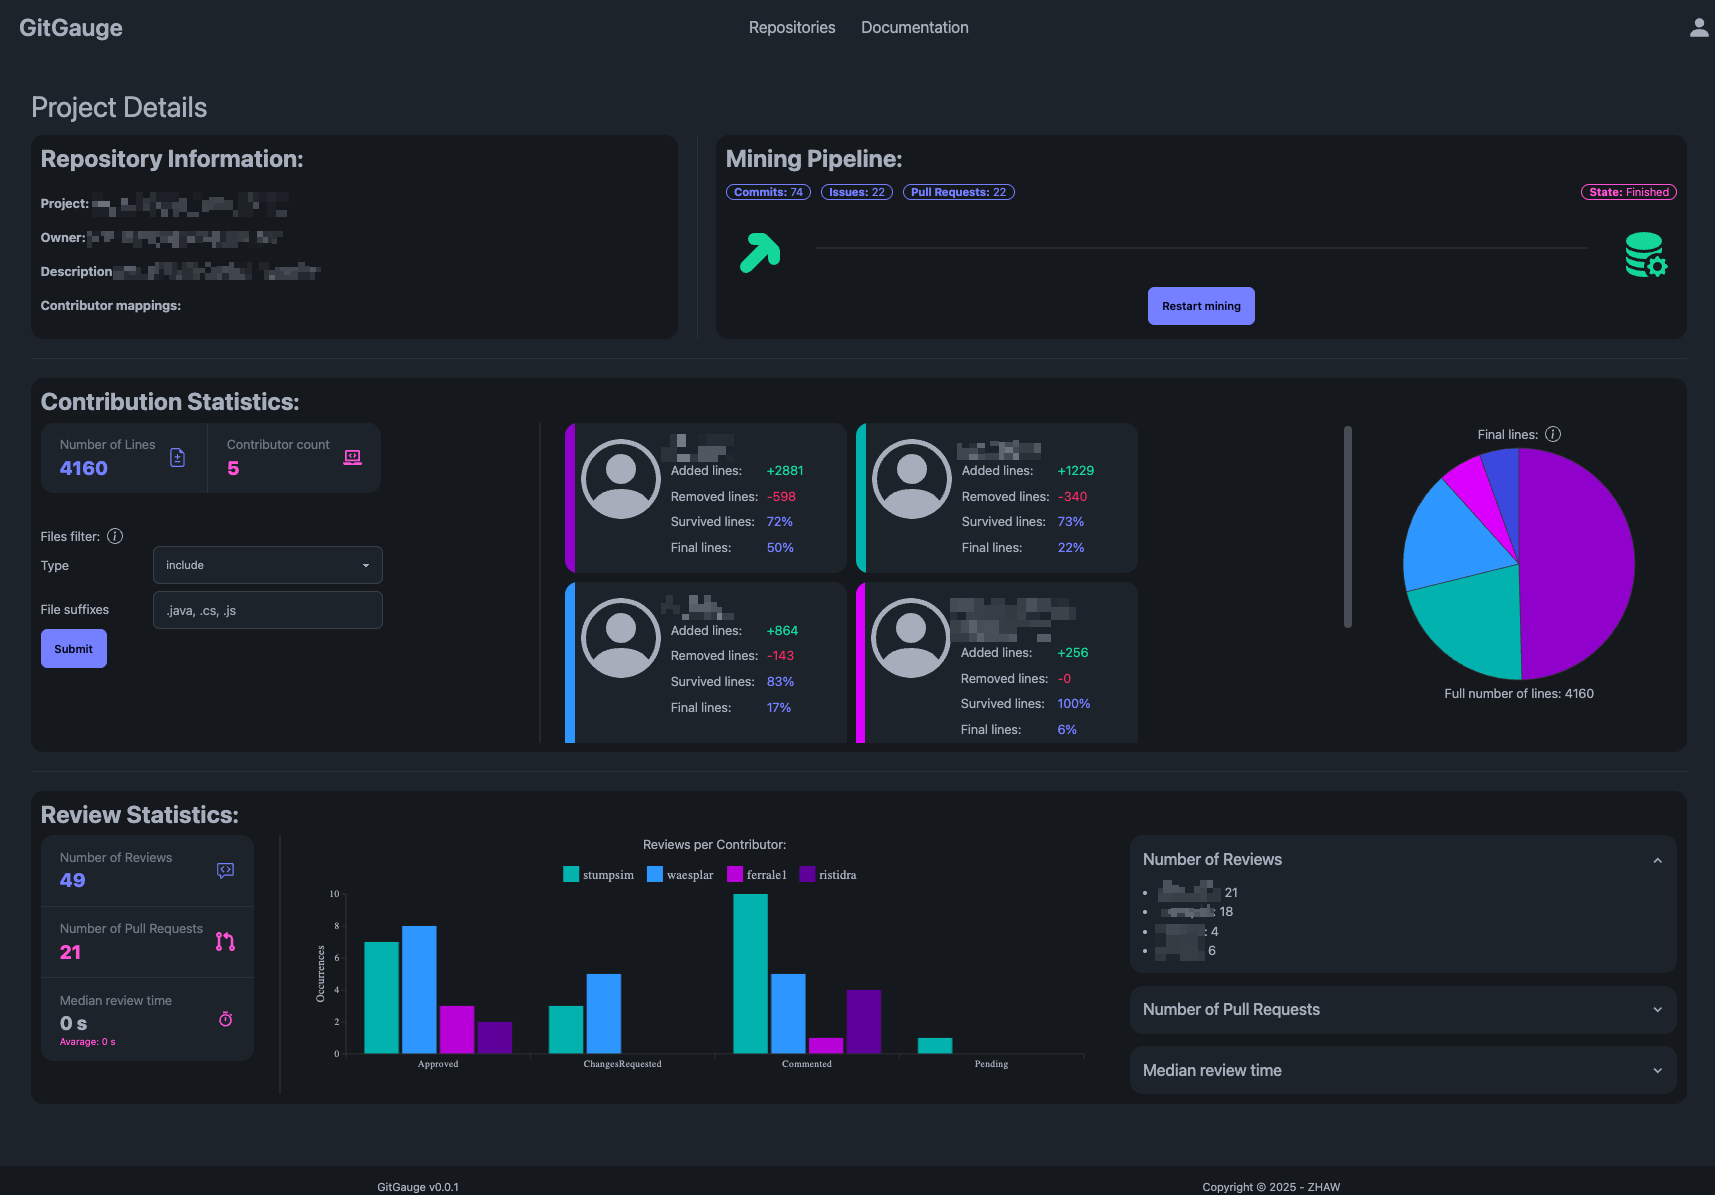
\includegraphics[width=0.8\textwidth]{Figures/giggauge-overview.png}
    \caption{Übersicht eines Projektes in GitGauge}
    \label{fig:gitgauge-project-overview}
\end{figure}

\newpage

\section{Aufgabenstellung}
Produktivitätsmetriken sollen aus Git-Repositories gewonnen werden. Aus den Daten der Repositories sollen aussagekräftige Kennzahlen für die Softwareentwicklung abgeleitet werden. Dies soll durch eine Literaturrecherche bestehender Metriken und die Entwicklung von Analysealgorithmen erfolgen.
Die offizielle Aufgabenstellung, gestellt von Michael Wahler, befindet sich im Anhang \secref{sec:OffAufgabenstellung}.
\newpage
\section{Forschungsfragen und Zielsetzung}
\label{sec:Zielsetzung}

Ziel dieser Arbeit ist es, Pull-Requests aus Projekten zu untersuchen und deren Eigenschaften hinsichtlich verschiedener Einflussfaktoren zu analysieren. Dabei stehen folgende Forschungsfragen im Vordergrund:

\forschungsfrage{forschungsfrage1}{
Besteht ein Zusammenhang zwischen der Latency eines Pull-Requests (Zeit bis zum Merge oder Schliessung) und dem Churn (Anzahl geänderter Codezeilen) des jeweiligen Pull-Requests?
}

\forschungsfrage{forschungsfrage2}{
Können die Schliessungsgründe der PRs in den Projekten ermittelt und klassifiziert werden?
}

\forschungsfrage{forschungsfrage3}{
Besteht ein Zusammenhang zwischen dem Zeitpunkt im Projektverlauf und der Review-Dauer von Pull-Requests?}


\forschungsfrage{forschungsfrage4}{
Lassen sich Patterns der Zusammenarbeit im Team erkennen, hinsichtlich der Tage, an denen die Studierenden an den Projekten arbeiten?
}

\forschungsfrage{forschungsfrage5}{
Welche Unterschiede zeigen sich in der Nutzung von Pull-Requests zwischen Teilzeit- und Vollzeitstudierenden hinsichtlich Anzahl, Umfang und Dauer?
}

\forschungsfrage{forschungsfrage6}{
Welche Unterschiede zeigen sich in den Repository-Metriken zwischen den Studentenprojekten und professionellen GitHub-Organisationen?
}

\section{Übersicht der Arbeit}
Im \autoref{Chapter2} \textit{\nameref{Chapter2}} wird das theoretische Wissen vermittelt, welches für das Verständnis dieser Arbeit notwendig ist. Dabei wird auf  Git / GitHub-spezifische Methodiken eingegangen, die untersuchten Projekte erläutert und das als Grundlage dienende Tool GitGauge erklärt.

Das \autoref{Chapter3} \textit{\nameref{Chapter3}} beschreibt die Methodik der Arbeit. Es erläutert die Vorgehensweise und beschreibt die notwendigen Metriken zur Klärung der Forschungsfragen. Des Weiteren wird die Datengrundlage aufgezeigt.


Die Ergebnisse werden im \autoref{Chapter4} \textit{\nameref{Chapter4}} dargelegt. Dabei wird auf die spezifischen Forschungsfragen eingegangen und die Analysen zur Beantwortung der Fragen dargestellt. Zusätzlich wird die Erweiterung an der GitGauge-Applikation demonstriert.

Zum Schluss folgt das \autoref{Chapter5} \textit{\nameref{Chapter5}}, in dem noch einmal auf die Forschungsfragen und deren Ergebnisse eingegangen und diese bewertet werden. Ausserdem werden mögliche Erweiterungen aufgezeigt.





